\documentclass[11pt, oneside]{article}   	% use "amsart" instead of "article" for AMSLaTeX format
\usepackage{geometry}                		% See geometry.pdf to learn the layout options. There are lots.
\geometry{letterpaper}                   		% ... or a4paper or a5paper or ... 
\usepackage{graphicx}				% Use pdf, png, jpg, or eps§ with pdflatex; use eps in DVI mode
								% TeX will automatically convert eps --> pdf in pdflatex		
\usepackage{amssymb}
 
\usepackage[]{algorithm2e} 			% for the pseudocode

\date{}							% Activate to display a given date or no date
\parindent 0in
\parskip 6pt


 
\begin{document}

\title{\bf Glacier Growth Model \\
\vskip 0.5in
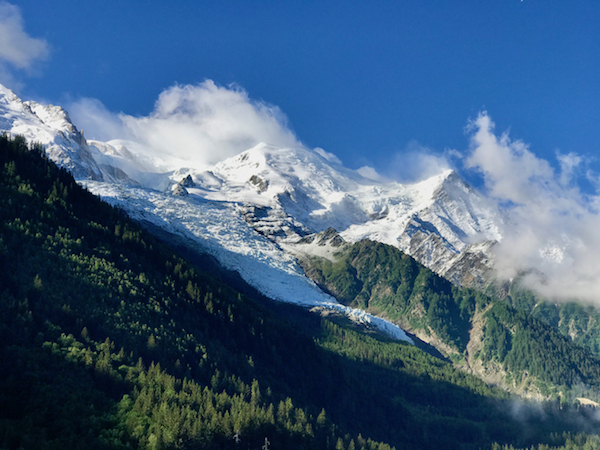
\includegraphics[width=.8\textwidth]{IMG_4569.jpg}
}

\maketitle
 
\section*{Learning Goals}
In this lecture we will use conservation of mass to build a simple model of a valley glacier growing through time.   You will learn about:
\begin{itemize}
\item glacier growth through snow accumulation and loss from melting and sublimation 
\item  glacier movement through internal deformation  and basal sliding 
\item  modeling the time dependent growth of the glacier
\end{itemize}

\section*{Overview}

The first step is to understand how glaciers grow and evolve in shape. Glaciers gain mass by the deposition of snow on the top surface and lose mass through the top surface by a combination of melt and sublimation.  The rate of snowfall and loss is primarily a function of the elevation.  The higher up you are, the more snow.  The lower you are, the more melt and sublimation.  

The Equilibrium Line Altitude (ELA) defines the elevation above which there is more snow gain than loss and below which there is more loss than snow gain.  If this were the only process occurring, you would have runaway growth of a glacier above the ELA and never find glaciers below the ELA.  This doesn't occur because glacier ice also moves.  

Glaciers move (or flow) in two main ways:  deformation of the ice and basal sliding of the ice along the base.

In order to build a glacier, we will quantify these rates of ice loss and gain from snow, melt, sublimation, ice deformation and basal sliding.  We will begin with a valley floor elevation profile with no snow, then slowly add snow through time and calculate the evolution of the glacier profile as it grows and moves.

\begin{figure}[htbp]
\begin{center}
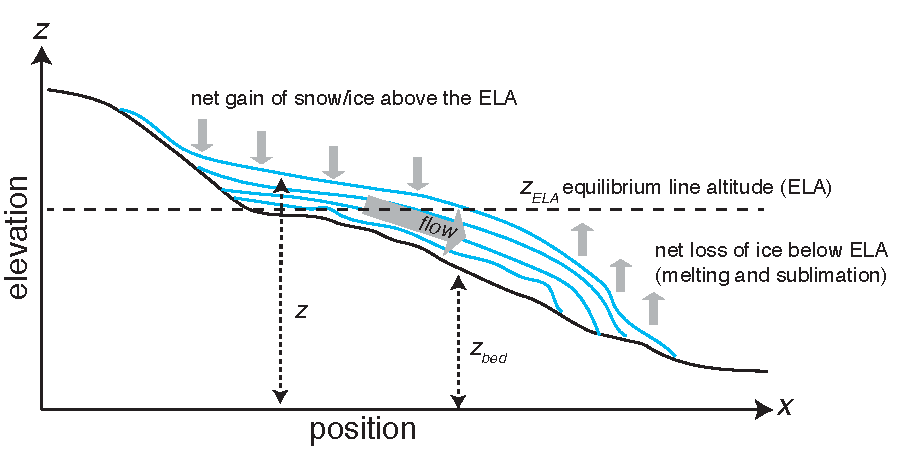
\includegraphics[width=.9\textwidth]{glacier.pdf}
\caption{Valley glacier cross section. Blue lines show the growth of the glacier over time due to mass increase above the equilibrium line altitude (ELA), downhill sliding, internal deformation,  and mass loss below the ELA. }
\label{default}
\end{center}
\end{figure}

%------------------------------------------------------------------------------------------
\section*{Basal Shear Stress} 
%------------------------------------------------------------------------------------------

\begin{figure}[htbp]
\begin{center}
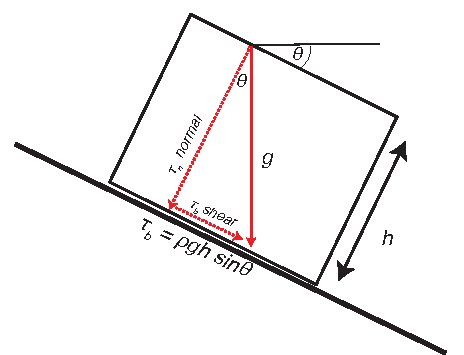
\includegraphics[width=.6\textwidth]{basal.pdf}
\caption{Stress due to the force of gravity $g$ for an ice block with density $\rho$ and thickness $h$.  The downward gravity vector, and the resulting stress vector, can be broken up into a component normal to the slope and one parallel to the slope. The parallel component of stress is known as the basal shear stress $\tau_b$ and depends on the slope angle $\theta$.}
\label{fig:Basal}
\end{center}
\end{figure}

The stress at the bottom of the glacier is the force per unit area on the base of ice.   The force is described by Newton's second law, $F= m a$ after inserting the value of Earth's gravity $g$ for the acceleration, thus $F=mg$ where  $g = 9.81$ m/$s^2$. The mass of the ice block is its density times its volume: $m = \rho A h$ where $\rho$ is the ice density, $A$ is the area of the base of the ice block and $h$ is the height.  For a flat lying block of ice, the stress is in the vertical direction due to gravity:
\begin{eqnarray}
	\tau_n = F/A =\rho g h.
\end{eqnarray}
$\tau_n $  has units of Pa (which is kg /(ms$^2$)).

What happens when the ice block is tilted, as it is for glaciers flowing down the sides of a mountain or sloping valley? This is shown schematically in Figure \ref{fig:Basal}. In this case the force of gravity can be divided into two vector components that can be found from trigonometry: one is  parallel to the ice bed and the other  is perpendicular.    For a slope angle $\theta$, the normal component $g_\perp = g \cos \theta$ while the parallel component is $g_\parallel = g \sin \theta$.   The parallel component of gravity  creates what is know as basal shear stress $\tau_b$ along the glacier bed. The basal shear stress is simply the parallel force per unit area on the glacier bed:
\begin{eqnarray}
	\tau_b = F_\parallel/A =\rho g_\parallel h = \rho g h \sin \theta.
	\label{eq:taub}
\end{eqnarray}

Due the basal shear stress, the glacier will slide along its bed. In our model, we will assume the velocity of the base of the glacier has the form
\begin{eqnarray}
	u_s = C_1  \tau_b^2 / (\rho g h) 
	\label{eq:us}
\end{eqnarray}
where $C_1$ is the sliding coefficient (m/(Pa yr)).  

When coding this up, be careful to avoid dividing by 0 when $h=0$. You can either write your code to carefully avoid this, or you can insert  the formula for $\tau_b$ to see that $u_s = C_1 \rho g h \sin^2\theta
$. With that equivalent form, $u_s$ is safely equal to $0$ when $h=0$ (i.e if the ice thickness is zero, there is no velocity).  Dividing by 0 is a common problem in computer modeling codes, so when possible, look for substitutions or rearrangements of a given formula that will avoid dividing by any variables that could be zero.

\begin{figure}[htbp]
\begin{center}
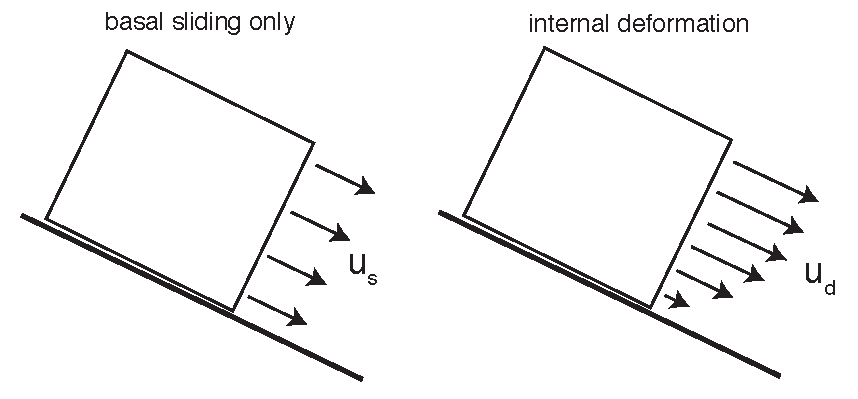
\includegraphics[width=.8\textwidth]{sliding_deformation.pdf}
\caption{Motion of the glacier occurs due to both basal sliding (left) and internal deformation (right).}
\label{fig:sliding}
\end{center}
\end{figure}


In addition to  basal sliding, the shear stress within the glacier will allow it to deform  plastically.  This is shown in Figure \ref{fig:sliding}.  The internal deformation is greatest near the base of the glacier where the pressure is highest. However, since all the material on top is rafted along when the lower parts of the glacier deform, the net movement is greatest on the upper half of the glacier. In our model we will use a simple formula for the deformation velocity averaged over the thickness of the glacier:
\begin{eqnarray}
	u_d = 0.4  A h \tau_b^3
	\label{eq:ud}
\end{eqnarray}
where $ A$ is the Arrhenius constant (Pa$^{-3}$yr$^{-1}$).  

The total lateral velocity of the glacier is the sum of the basal sliding and internal deformation velocities:
\begin{eqnarray}
	u = u_d + u_s
\end{eqnarray}
Using the definition of $u_d $ and $u_s$ above, our velocity has units of m/yr.

%------------------------------------------------------------------------------------------
\section*{Fluxes} 
%------------------------------------------------------------------------------------------
\begin{figure}[htbp]
\begin{center}
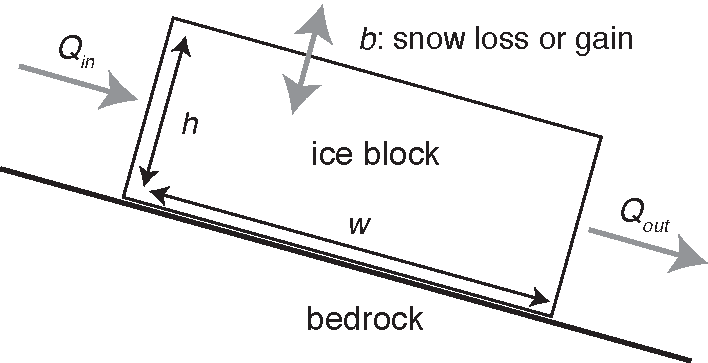
\includegraphics[width=.6\textwidth]{block.pdf}
\caption{Control volume for the glacier growth model.}
\label{controlVolume}
\end{center}
\end{figure}

To understand the flux at a given location on the glacier, consider the control volume shown in Figure \ref{controlVolume}.  $Q_{in}$ and $Q_{out}$ represent the flux of material into and out of the control volume due to sliding and deformation. $b$ represents the addition or subtraction of material on the top part of the glacier due to accumulation or ablation.

We will assume a model where mass is added to or subtracted from the top surface of the glacier as a function of position. Above the equilibrium line, volume is added due to snowfall, whereas below the ELA volume is loss due to melting and sublimation. We parameterize this as:
\begin{eqnarray}
	b(x) = 0.005 (z- z_{ela}) 
	\label{eq:b}
\end{eqnarray}
where here in our 2D problem $b$ will have units of m/yr. $b$ is positive above $z_{ela}$ and is negative below.  In our homework, we will restrict $b$ to have a maximum value of 2. This means we limit the maximum amount of ice gain due to snowfall to be 2 m/yr, which seems reasonable (also note that ice has a density nearly twice that of snow due to compaction, so this implies a maximum snowfall of about 4 m/yr).

At a given location, we can compute the flux $Q$ that is lost due to sliding and deformation:
\begin{eqnarray}
	Q = -h ( u_s + u_d)
	\label{eq:Q}
\end{eqnarray}
Note that  since $h$ has units of meters, $Q$ has units of m$^2$/yr.  Note also the negative sign on the formula for $Q$, which implies that material is lost due to the sliding and deformation.   So the value of $Q$ in a given location is flux of material moving downhill at that location. However, there is continuum of flux along the glacier, and so at a given spot, ice will move away in the downhill direction, but ice will also flow into that spot from further uphill.  This is represented by $Q_{out}$ (loss) and $Q_{in}$ (gain) in Figure \ref{controlVolume}. 

\begin{figure}[htbp]
\begin{center}
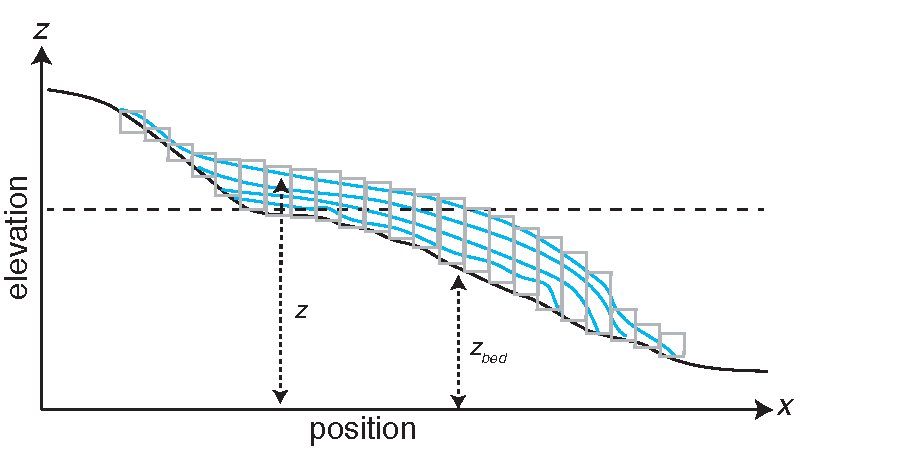
\includegraphics[width=.8\textwidth]{glacier_volumes.pdf}
\caption{Breaking the glacier model up into a series of control volumes (gray boxes) which will be used to conserve mass as a function of time. The width of each cell is fixed but its height will vary as a function of time.}
\label{fig:volumes}
\end{center}
\end{figure}

\begin{figure}[htbp]
\begin{center}
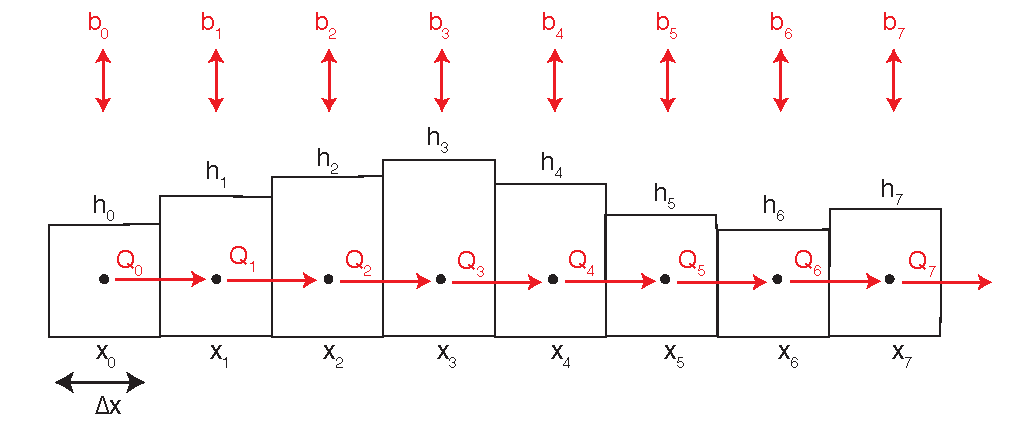
\includegraphics[width=.8\textwidth]{cells.pdf}
\caption{A close up view of the control volume cells. The cells are located at positions $x_0,x_1,x_2,x_3,...$ with fixed width $\Delta x$ and have associated ice thicknesses $h_0,h_1,h_2,h_3,...$ .  $h$ for each cell can vary over time. $Q_i$ represents the flux (m$^2$/yr) of ice out of cell $i$ and into cell $i+1$. Thus the net flux in cell $i$ is $\Delta Q_i =  Q_i - Q_{i-1}$.   The thickness $h$ can also change due to material being added or subtract to the top of the ice in each cell through the snowfall/snowmelt function $b$. {\it Note that for ease of explanation, the topographic profile has been flattened here}. }
\label{fig:cells}
\end{center}
\end{figure}

Now that you have an understanding of the control volume, we can divide up the model into a series of control volume cells with fixed width $\Delta x$ as shown in Figures \ref{fig:volumes} and \ref{fig:cells}. The cells are located at positions $x_0,x_1,x_2,x_3,...$ and have associated ice thicknesses $h_0,h_1,h_2,h_3,...$ . These control volumes are fixed in location, and the glacier will flow from one volume cell to the next.  Thus we can balance the mass fluxes $Q$ between them.  In your homework assignment,  $h$ starts at zero for every cell; over time as ice fluxes through the cell, and as ice is also added or subtracted by snowfall or melting, $h$ will change. The only limit we impose is that $h\ge 0$, meaning the model can't have a negative thickness of ice! 

Inspection of Figures \ref{fig:cells} shows that $Q_i$ represents the flux (m$^2$/yr) of ice out of cell $i$ and into cell $i+1$.  But cell $i$ will also gain ice from the cell to its left through flux $Q_{i-1}$. Thus the net flux in cell $i$ is 
\begin{eqnarray}
	\Delta Q_i =  Q_i - Q_{i-1}.
	\label{eq:deltaQ}
\end{eqnarray}
Note the order of $Q_i$ and  $Q_{i-1}$ here, which agrees with our early definition of $Q$ in equation \ref{eq:Q} being the flux out of a given region.

Since the cell width is fixed, the net gain or loss represented by $\Delta Q_i $ leads to a change in height $h_i$ per unit time of $\Delta Q_i/\Delta x$. Each cell also gains or loses height from the snowfall/snowmelt  function $b$ given in equation \ref{eq:b}.    Since $Q$ and $b$ are rates (i.e., the change in something per unit time), we can define a time step length $\Delta t$ and then compute the total change in height of cell $i$ for that time step as:
\begin{eqnarray}
	\Delta h_i = (\Delta Q_i/\Delta x + b_i )\Delta t,
	\label{eq:h_update}
\end{eqnarray}
where $\Delta t$ has units of years here.

%------------------------------------------------------------------------------------------
 \section*{Physics Review}
 %------------------------------------------------------------------------------------------
 Before we talk about how to write a time lapse glacier simulation code, let's review what we have learned from the physics above.
 \begin{enumerate}
\item The basal shear stress $\tau_b$ depends on the slope $\theta$ of the top of the glacier as well as its thickness. See equation \ref{eq:taub}.
\item The sliding velocity and internal deformation velocities will increase rapidly with increasing $\tau_b$. See equations \ref{eq:us} and \ref{eq:ud}. Therefore, we expect the fastest velocities on the steepest slopes (that makes sense) but also where the ice is thicker.
\item The ice flux $Q$ (area/yr) in a given spot is proportional to the ice thickness at that spot and its total velocity $u_s + u_d$. See equation \ref{eq:Q}. Thus we expect this to be greatest for thick ice on steep slopes and smallest on flat or low slopes.
\item The net flux at a given location is equal to the difference of the outgoing and incoming flux. This is just conserving mass, or in our specific case, the equivalent conservation of the total cross sectional area of ice (in the vertical plane). See equation \ref{eq:deltaQ}.
\item Ice can also be added or lost at a given location due to snowfall or melting. See equation \ref{eq:b}.
\item For a given control volume cell, the total change in the height of the glacier there depends on the net flux $\Delta Q$, the local snowfall or melt  rate $b$ and the length of the time step taken. See equation \ref{eq:h_update}.
\end{enumerate}

 
%------------------------------------------------------------------------------------------
 \section*{Time Stepping  Code Outline}
 %------------------------------------------------------------------------------------------
 
Now let's consider how to put all this information together so that you can write a modeling code that will simulate the time evolution of a growing glacier.  A pseudocode outlining the procedure is shown in Algorithm \ref{pseudocode} below.

To compute the slope at each location, you can use the finite difference approximation:
\begin{eqnarray}
\theta_i = \arctan(-\Delta z_i /\Delta x)
\end{eqnarray}
 The slope angle should be positive clockwise down from horizontal. Here $\Delta z_i$ is the difference in the height of the top of the glacier between cell $i+1$ and cell $i$. For $n$ cells, this will only give you $n-1$ values for $\theta$; you can append the last value (i.e. repeat the last value) so your $\theta$ array has $n$ values.  Also, the slope is for the top of the glacier, so use $z$ when computing it, NOT $z_{bed}$ or $h$ alone.

\begin{algorithm}[H]
\label{pseudocode} % add a label for \ref{} commands later in the document
	Inputs:
 \begin{itemize}
\item $x$, $z_{bed}$ - topography profile arrays  with even spacing $\Delta x$. [m]
\item $z_{ela}$   - the equilibrium line altitude [m]
\item $\rho$  - ice density [kg/m$^3$]
\item $A$ - Arrhenius constant for ice. [Pa$^3$/yr]
\item $C_1$ - ice sliding coefficient. [m Pa$^{-1}$ yr$^{-1}$]
\item $\Delta t$ - time step length [yr]
\item  $t_{max}$ - maximum length of time to run the simulation for [yr]	
\end{itemize}
Initialize arrays $h = 0$  and $z = z_{bed} + h$, where $h$ and $z$ have the same number of elements as $x$.\\
 $t = 0$ \\
    \While{$t \le t_{max}$}{  
	Compute $\theta, \tau_b, u_s, u_d, Q$ and $b$ for each cell. Limit $b$ so that  $b \le 2$. \\
	Compute $\Delta Q_i$ for each cell. Note for the first cell: $\Delta Q_0 = Q_0$ \\
	Compute $\Delta h_i$ for each cell. \\
	Update $h$: $h = h + \Delta h$. Limit $ h$ so that $h \ge 0$. \\
	Update $z$: $z = z_{bed} + h$. \\
	$t = t+\Delta t$ \\
	}
 \caption{Glacier growth modeling pseudocode}
\end{algorithm}




\end{document}  